\chapter{Introdução}
\label{cap:introducao}
%=====================================================

Este Relatório de Estágio.....

\section{Exemplo de figura}

\begin{figure}[ht]
	\centering
	\caption{Exemplo de figura.}
	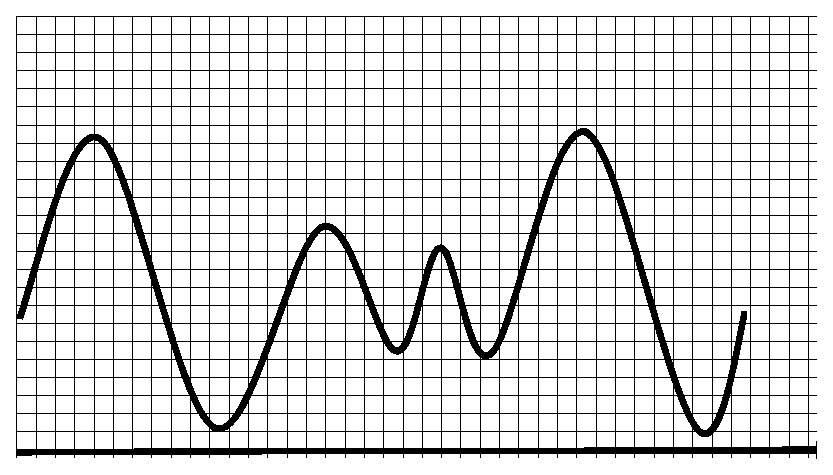
\includegraphics[width=0.5\textwidth]{fig/figexemplo.eps}
	\label{fig:figexemplo}
\end{figure}


\section{Exemplo de tabela}

\begin{table}[ht]
	\centering
	\caption{Exemplo de tabela.}
	\label{tab:exemplo}
	\begin{tabular}{|c|c|c|}
		\hline
		\textbf{Coluna 1} & \textbf{Coluna 2} & \textbf{Coluna 3} \\ \hline
		Linha 1 & Valor 1 & Valor 2 \\ \hline
		Linha 2 & Valor 3 & Valor 4 \\ \hline
	\end{tabular}
\end{table}

\section{Exemplos de citações}

Nesta seção são apresentados alguns exemplos de como realizar citações. Note que podem ser utilizados as macros \verb|\citet| e \verb|\cite|. A macro \verb|\citet| é utilizada para citar referências no formato de texto normal, em que o nome do autor (ou autores) e o ano da publicação são apresentados no texto. A macro \verb|\cite| é utilizada para citar referências entre parênteses, em que o nome do autor (ou autores) e o ano da publicação são apresentados dentro dos parênteses.

\subsection{Exemplo 1}
Neste ano, o Núcleo de Informação e Coordenação do Ponto BR (NIC.br), responsável pela administração e coordenação do domínio de topo ``.br'' da Internet, emitiu um alerta sobre a iminente escassez de endereços IPv4. Em 31 de janeiro, os últimos blocos disponíveis de endereços IPv4 foram distribuídos, incluindo para a região da América Latina e Caribe, da qual o Brasil faz parte. Estima-se que o Brasil ainda possua estoque de endereços IPv4 no padrão ``.br'' para distribuição por mais um ano, por meio do NIC.br \citep{nicbr2023IANA}.

\subsection{Exemplo 2}
O estudo de \citet{spanhol2015dataset} apresenta um conjunto de dados composto por 7.909 imagens de histopatologia de câncer de mama, obtidas de 82 pacientes, e disponíveis em uma plataforma pública. O conjunto de dados, disponibilizado em \url{http://web.inf.ufpr.br/vri/breast-cancer-database}, inclui imagens tanto benignas quanto malignas e é destinado à tarefa de classificação automatizada dessas imagens em duas classes. Essa ferramenta de diagnóstico auxiliado por computador pode ser valiosa para os clínicos. 

\subsection{Exemplo 3}

A utilização da lógica fuzzy combinada a técnicas analíticas pode ser uma abordagem eficaz para alcançar maior eficiência energética em dispositivos de redes de sensores sem fios (\textit{Wireless Sensor Networks} - WSNs). Essa abordagem propõe o uso de métodos eficientes de seleção de retransmissores para melhorar a vida útil da bateria, o desempenho e a eficiência energética das WSNs \cite{engel2013relay}.

\subsection{Exemplo 4}

Nos dias atuais, as tecnologias modernas de tecnologia da informação têm sido amplamente utilizadas com o objetivo de aprimorar a eficiência e o desempenho de sistemas de produção e de rede. Essas tecnologias, como Internet das Coisas (IoT), Redes de Funções Virtuais (NFV), Aprendizado de Máquina e outras, têm sido aplicadas em diversos contextos, desde manufatura aditiva (impressão 3D) até gerenciamento de redes de telecomunicações. Essas abordagens inovadoras visam obter ganhos significativos em termos de otimização de processos, monitoramento em tempo real, detecção de falhas, automação e tomada de decisões baseada em dados \cite{huff2020building,scheffel2021automated}. 

